\section{Histogram}
In this section the histograms of the attributes will be covered. In the next section the boxplots for the attributes are explained. The attributes will be explained in details there.
\begin{figure}[H]
\centering
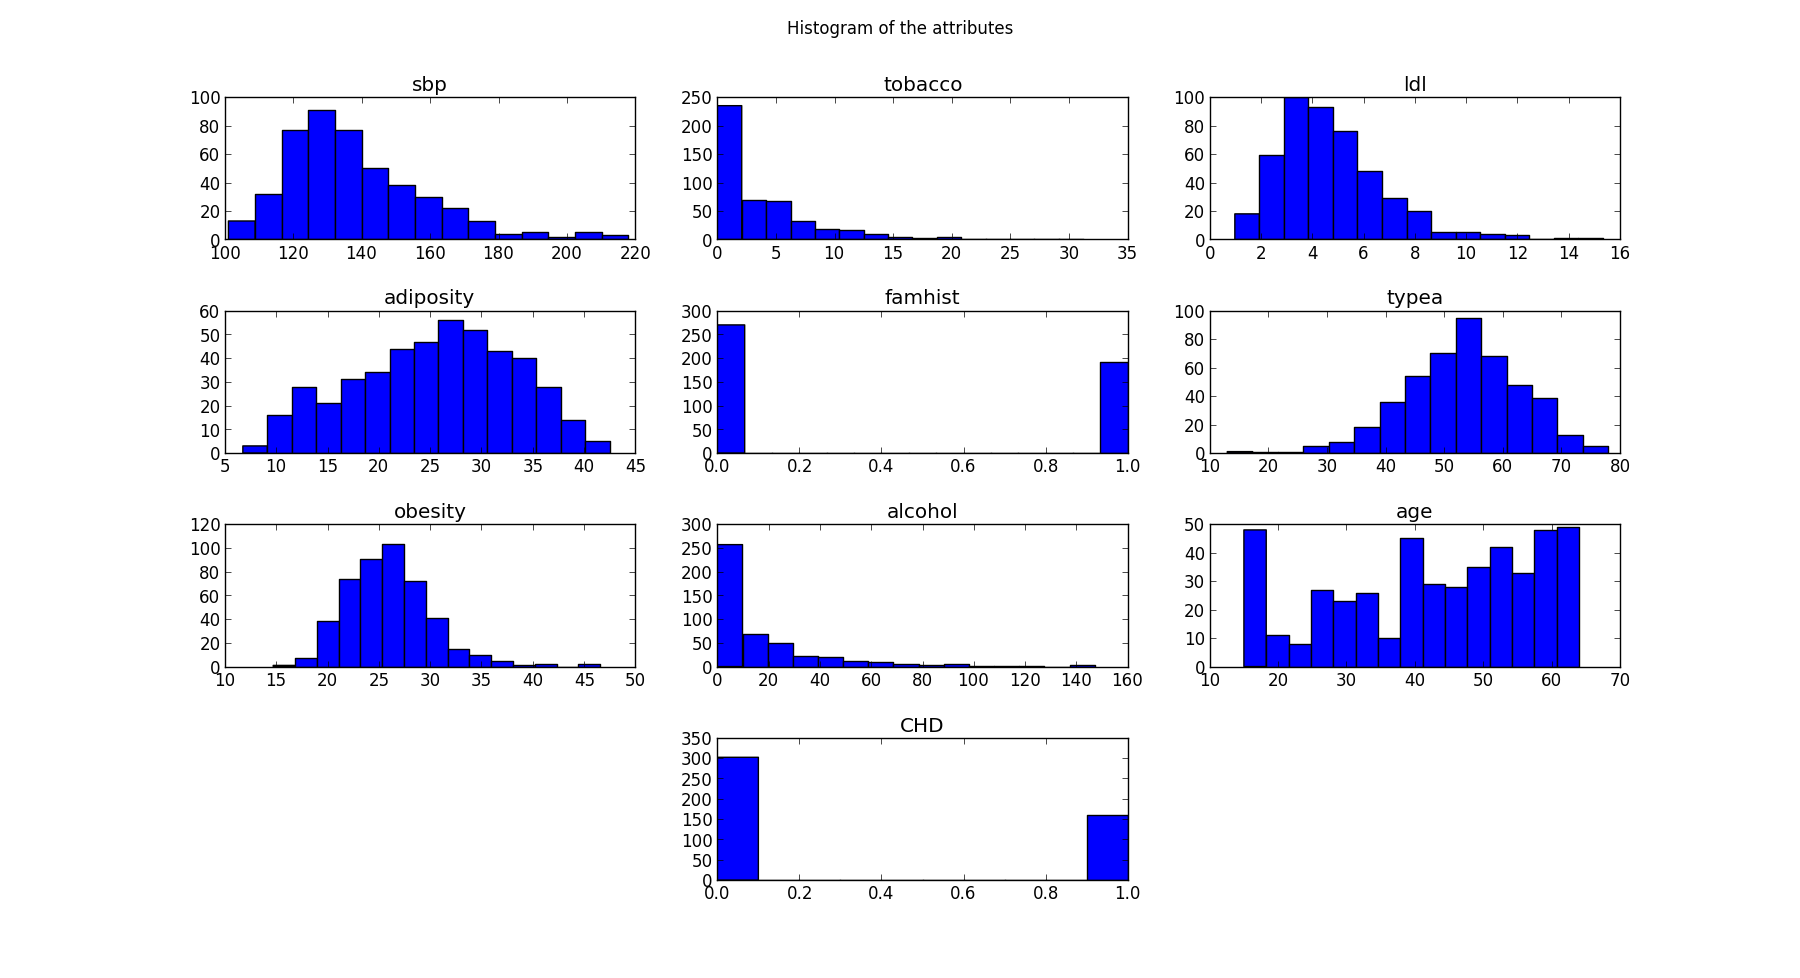
\includegraphics[width=12cm, keepaspectratio=true]{pictures/histogram.png}
\caption{\footnotesize Histograms}
\label{histogram}
\end{figure}
Several of our attributes seem to be close to normally distributed. These are:
\begin{itemize}
\item SBP - Systolic Blood Pressure
\item ldl - low density lipoprotein cholesterol
\item typeA
\item Adiposity
\item Obesity
\end{itemize}
\paragraph{Adiposity and Obesity}
The latter two, Adiposity and obesity are closely connected, since they both concern the size of the body. How closely connected they are will be explained later.

\paragraph{Type A} is an index of aggresiveness and stresslevel of the person. This is very normally distributed, and peaks at around 55.

\paragraph{SBP - Systolic Blood Pressure} 	seems to be peaking at around 130, which is considered a little bit high, but since the SBP is rising as you get older, and the average age of our dataset is over 40, this seems reasonable. The curve is extending far to the right, which will be covered in the next section covering the boxplot.

Those attributes not distributed normally:
\begin{itemize}
\item Tobacco
\item Famhist
\item Alcohol
\item Age
\item CHD
\end{itemize}

\paragraph{Tobacco} indicates that most persons in the dataset does not smoke.
\paragraph{Famhist} Is a binary attribute. Showing a few more people in the dataset does not have any family members with CHD, than who does have family history with CHD.
\paragraph{Alcohol} looks a lot like tobacco. How closely related they are will be shown later.
\paragraph{Age} is ranging from 15 to 65, and shows there are more data from people older than 40.
\paragraph{CHD} is quite important, because this shows us that there are around 300 cases of people \textit{not} having the CHD disease, while only 160 \textit{does} have the disease. This does have an influence in the scatterplots explained later.